% Scenario 1: Usability Enhancement through Standardized UIs
\begin{table}[H]
    \centering
    \begin{tabularx}{\textwidth}{@{} lX @{}}
    \toprule
    \textbf{Aspect} & \textbf{Details} \\
    \midrule
    Source & Passenger interacts with the payment terminal UI. \\
    Stimulus & The passenger navigates the options to buy a ticket. \\
    Artifact & Standardized User Interface (UI) of the payment terminal. \\
    Response & The UI displays a clear, consistent, and intuitive navigation path for ticket purchase. \\
    Measure & 95\% of passengers successfully purchase tickets without assistance. \\
    \bottomrule
    \end{tabularx}
    \caption{Scenario for Usability - Standardized UIs}
    \label{table:usability_enhancement}
\end{table}


% Scenario 2: Scalability via Tycoon API
\begin{table}[H]
    \centering
    \begin{tabularx}{\textwidth}{@{} lX @{}}
    \toprule
    \textbf{Aspect} & \textbf{Details} \\
    \midrule
    Source & A new tycoon's system attempting to integrate with the TrIP system. \\
    Stimulus & The tycoon sends a request to access route and fare data. \\
    Artifact & Tycoon API that standardizes data exchange with the TrIP system. \\
    Response & The API facilitates the integration, providing access to the required data. \\
    Measure & Integration is completed within 3 business days, with zero errors in data format conversion. \\
    \bottomrule
    \end{tabularx}
    \caption{Scenario for Scalability via Tycoon API}
    \label{table:scalability_tycoon_api}
\end{table}

% Scenario: Payment Flexibility for Diverse User Groups
% Scenario: Accommodating Varied Payment Preferences
\begin{table}[H]
    \centering
    \begin{tabularx}{\textwidth}{@{} lX @{}}
    \toprule
    \textbf{Aspect} & \textbf{Details} \\
    \midrule
    Source & Passengers with varying preferences for payment, each approaching the transit system's access points. \\
    Stimulus & Passengers select their payment method of choice, ranging from physical cash for single rides to digitally managed subscriptions, and some opt for the convenience of pre-loaded fare cards. \\
    Artifact & Integrated payment and authentication platform within the TrIP system. \\
    Response & The system adeptly manages the assortment of transactions, crediting cash payments, verifying subscription validity, and debiting pre-loaded cards, all in a streamlined fashion. \\
    Measure & The system consistently processes transactions of all types with a rapid response rate, registering a less than 2-second average processing time and maintaining a transaction success rate of 99\%. \\
    \bottomrule
    \end{tabularx}
    \caption{Scenario for Usability via Accommodating Varied Payment Preferences}
    \label{table:varied_payment_preferences}
\end{table}

\section{Functional Viewpoint}\label{sec:functional}

We start discussing the Functional Viewpoint by analyzing stakeholder concerns that need to be addressed.
We individuated the following user stories:
\begin{itemize}[noitemsep]
    \item \userStoryOne
    \item \userStoryFour
    \item \userStorySix
    \item \userStorySeven
    \item \userStoryNine
    \item \userStoryTen
    \item \userStoryTwelve
    \item \userStorySixteen
    \item \userStoryTwenty
    \item \userStoryTwentySix
    \item \userStoryTwentySeven
    \item \userStoryThirtyNine
    \item \userStoryFortyOne
  \end{itemize}
  

As a consequence, we decided to prioritize Quality Attributes for this view as indicated in Table~\ref{tab:functional_view}.
\begin{table}[h!]
    \centering
    \resizebox{\textwidth}{!}{%
    \begin{tabular}{|l|c|c|c|c|c|c|c|c|c|}
      \hline
      & Usability & Performance & Security & Modifiability & Cost Efficiency & Availability & Safety & Integrability & Maintainability \\
      \hline
      Functional View & 
      \cellcolor{gray!60}X & % Usability (2nd priority)
      \cellcolor{gray!40}X & % Performance (3rd priority)
      & & 
      \cellcolor{gray!55}X & % Cost (3rd priority)
      & % Availability (4th priority)
      & 
      \cellcolor{gray!20}X& 
      \cellcolor{gray!90}X \\ % Maintainability (1st priority)
      \hline
    \end{tabular}
    }
    \caption{Functional View Prioritized Quality Attributes}
    \label{tab:functional_view}
\end{table}


\subsection{View: Main Functional Elements}

\subsubsection{Model}

\begin{figure}[H]
    \centering
    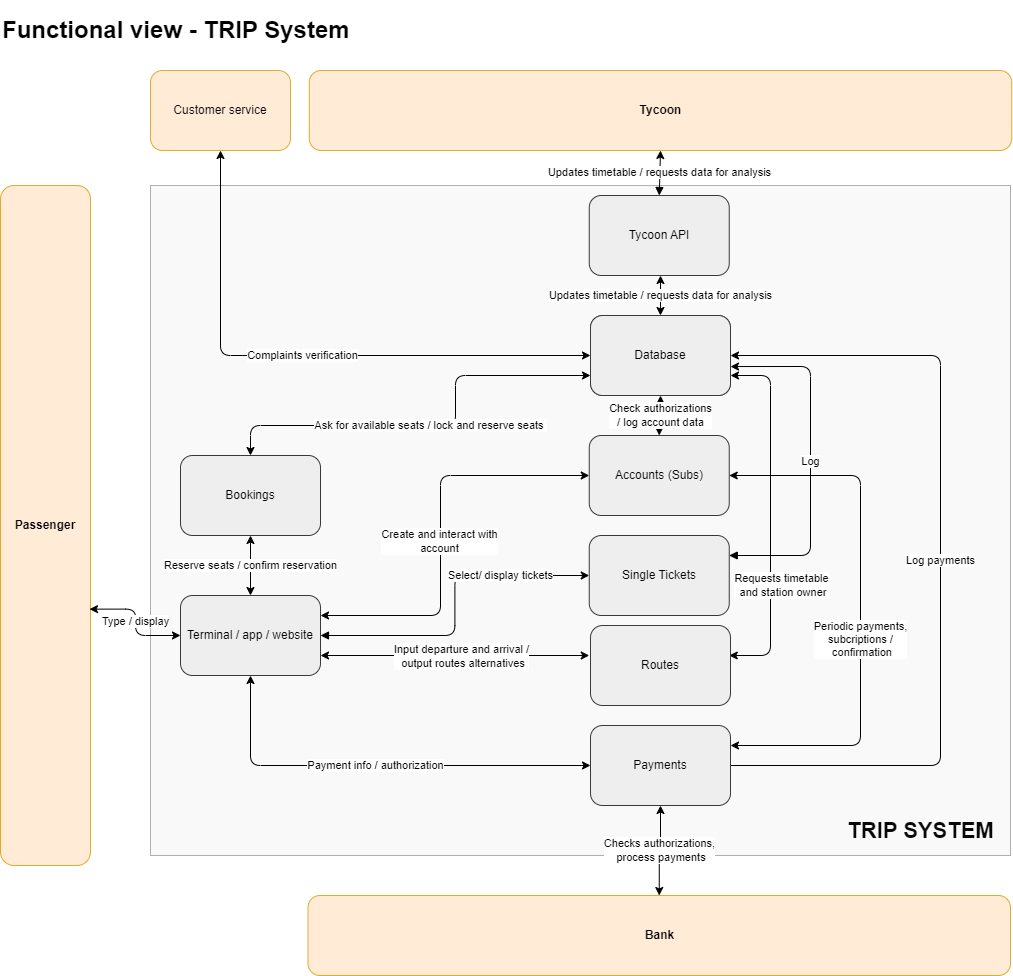
\includegraphics[width=\textwidth]{drawings/views_final_version/functional_view.png}
    \caption{TrIP System.}
    \label{fig:trip_system}
\end{figure}

\subsubsection{Description}
The functional view diagram of the TrIP system illustrates the major functions of the system and how they interact with each other. The diagram features boxes representing different functions, connected by arrows that represent interactions.
The system starts with the passenger, who can interact with the system through various interfaces, such as terminals, apps, or websites. The user can input their departure and arrival stations, and the system will then display a list of available routes. The passenger can then select a route and proceed to payment.
The payment system can handle various payment methods, including single tickets, subscriptions, and fillable cards. If the passenger has a subscription, the system will automatically check if the subscription is valid for the selected route. This is done by the Account and Subscription Management module, which communicates with the tycoon systems to verify the subscription. If the subscription is not valid, the passenger will be prompted to purchase a single ticket or top up their fillable card.
Once the payment is processed, the system will generate a ticket or update the passenger's travel card.
The system also includes a number of other functions, such as a booking system, a route optimization system, and a customer service system. The booking system allows passengers to reserve seats on trains. The route optimization system helps passengers find the most efficient routes between their departure and arrival stations. The customer service system provides support to passengers with inquiries and complaints.
The system is designed to be scalable and flexible, so that it can be easily adapted to accommodate new tycoons and changing business models. The system is also designed to be secure, so that passenger data is protected from unauthorized access.

\subsubsection{Glossary of Elements}
\begin{table}[H]
    \centering
    \begin{tabular}{@{}clp{9cm}@{}}
    \toprule
    \textbf{Id} & \textbf{Name} & \textbf{Description} \\
    \midrule
    1 & Passenger & End-users of the TrIP SYSTEM who interact with various system components to manage their travel experience. \\
    2 & Customer Service & The interface for passengers to make inquiries or complaints and receive assistance with bookings or account issues. \\
    3 & Tycoon & The administrative or business logic module that updates timetables and analyzes system data for improvements or reporting. \\
    4 & Database & An abstraction for the set of databases that stores all system data including passenger accounts, bookings, and payment information. Detailed information about how different databases are handled is detailed in the Information View.\\
    5 & Bookings & The system component where passengers can inquire about seat availability and make reservations. \\
    6 & Accounts (Subs) & The system managing passenger accounts and subscriptions, responsible for authorization checks and account data logging. 
    It is is also responsible for single tickets and fillable cards, as they can be seen as temporary and anonymous accounts. \\
    7 & Routes & The component that manages route information and provides passengers with timetables, station ownership details, and route alternatives. \\
    8 & Payments & The module handling all financial transactions, including passenger payments and periodic billing. \\
    9 & Bank & The financial institution interface for authorizing and processing payments linked to the system. \\
    10 & Terminal/App/Website & User interfaces through which they can access services such as booking, route information, and payment. \\
    \bottomrule
    \end{tabular}
    \caption{Glossary of elements detailing the components of the TrIP SYSTEM and their roles in facilitating user interaction and service provision.}
    \label{tab:glossary_trip_system}
\end{table}

\subsubsection{Analysis on Perspectives}
In addressing the Quality Attribute (QA) priorities highlighted by users, our Main Functional Elements view incorporates several key decisions designed to enhance usability, maintainability, scalability, and performance efficiency. \\

\noindent \textbf{Scenarios}
\scenarioOneFunctional
\scenarioTwoFunctional

\noindent To meet the \textit{usability} needs of passengers, we have opted for standardized User Interfaces (UIs). These UIs, being open-source and widely utilized, benefit from a large user base that contributes to their \textit{maintenance} and robustness. This choice ensures a user-friendly and reliable interface for passengers over the long term. Furthermore, it aligns with the TrIP owner's preferences by offering ease of maintenance and \textit{low operational costs}.

In response to Event 1, which underscored the need for easier \textit{integration} of new tycoons, we have implemented the Tycoon API. This API standardizes data requests from each tycoon, irrespective of their mode of transportation, thus facilitating the smooth integration of new tycoons into the system. The Tycoon API, in conjunction with the accounts and bookings module, ensures that passengers can effortlessly utilize their subscriptions across different networks and book their preferred routes. Hence, implementation of Tycoon API increases the \textit{usability} and \textit{integrability} for the Tycoons.

Event 3, which focused on traffic jams, raised the importance of optimizing system \textit{performance} during peak periods. By deciding on a centralized route management module, we have streamlined data flow between the TrIP system and the tycoons. This module not only simplifies data management but also enhances the system's ability to handle high request volumes through optimization and caching strategies.

\subsection{View: Ticket scanning}
\subsubsection{Model}
\begin{figure}[H]
    \centering
    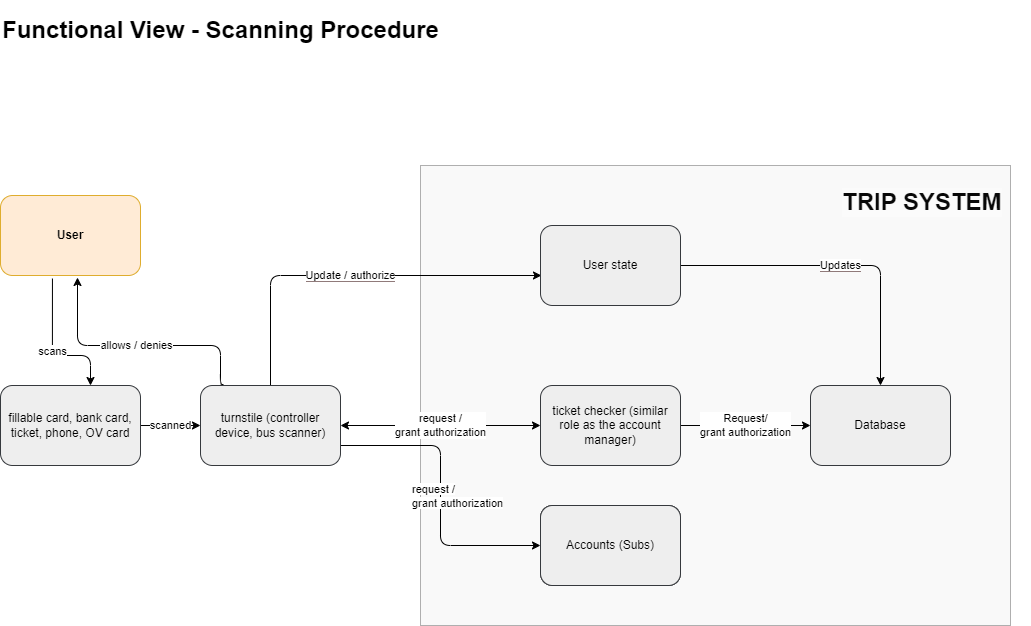
\includegraphics[width=\textwidth]{drawings/views_final_version/functional_view scanning.png}
    \caption{Interaction with a ticket scanner.}
    \label{fig:ticket_scanner}
\end{figure}

\subsubsection{Description}
The scanning procedure within the TRIP SYSTEM encapsulates the interactions between the passenger and the system's access control mechanisms. It begins with the passenger presenting a valid form of transit access—such as a card or mobile device—to a scanning device like a turnstile or bus scanner. This device then consults the Passenger State, a repository of the passenger's authorization status, to allow or deny entry. In parallel, the Ticket Checker function verifies the passenger's credentials against the Accounts subsystem, which manages detailed account information and subscriptions. Any changes to the passenger's state are updated in real time in the central Database, ensuring accurate tracking of access and travel history. This process ensures a secure, streamlined experience for passengers while providing the system with the necessary oversight to prevent unauthorized access

\subsubsection{Glossary of Elements}
\begin{table}[H]
    \centering
    \begin{tabular}{@{}clp{9cm}@{}} % Adjust the width of the description column as needed to fit the page
    \toprule
    \textbf{Id} & \textbf{Name} & \textbf{Description} \\
    \midrule
    1 & Passenger & The individual who uses the trip system and interacts with various components such as turnstiles and ticket checkers. \\
    2 & Fillable Card, Bank Card, Ticket, Phone, OV Card & Various forms of identification or payment methods that the passenger can use within the system. These are scanned by the turnstile to allow or deny access. \\
    3 & Turnstile (Controller Device, Bus Scanner) & A physical barrier or scanner that reads the passenger's ticket or card and determines whether to grant or deny access based on the passenger state or account information. \\
    4 & Passenger State & A system component that maintains the current state of the passenger within the system, including authorization and access rights, which is updated upon passenger interaction with the turnstile. \\
    5 & Ticket Checker (Account Manager) & An agent or system role similar to the account manager that requests or grants authorization for passenger access, potentially by checking the passenger state against the database. \\
    6 & Accounts (Subs) & The subsystem managing passenger accounts and subscriptions, which may interact with the turnstile and ticket checker to verify and update passenger access rights. \\
    7 & Database & An abstraction for the set of databases that stores all system data including passenger accounts, bookings, and payment information. Detailed information about how different databases are handled is detailed in the Information View.\\
    \bottomrule
    \end{tabular}
    \caption{Glossary of elements for the Functional View - Turnstiles, detailing the components and their roles in passenger access and authorization within the TrIP SYSTEM.}
    \label{tab:glossary_turnstiles}
\end{table}

\subsubsection{Analysis on Perspectives}
In addressing the Quality Attribute (QA) priorities highlighted by users, our ticket scanning view incorporates several key decisions designed to enhance usability, maintainability, scalability, and performance efficiency.

The introduction of multiple payment methods, including fillable cards, credit cards, and single tickets, significantly simplifies passenger interaction with the TrIP system. The integration of accounts and subscriptions further facilitates seamless travel across multiple tycoon networks, enabling passengers to efficiently manage and use their subscriptions.
\newline
\newline
\noindent \textbf{Scenarios}
\scenarioThreeFunctional

In summary, the functional viewpoint of our system meticulously addresses the initial QA priorities, along with the challenges presented by new tycoon integration (Event 1) and traffic jams (Event 3). These decisions collectively ensure a user-friendly, scalable, and high-performing TrIP system for passengers, tycoons, and the TrIP owner alike.